Machine learning (ML) is an increasingly popular data analytic technique widely employed in areas not limited to particle physics. It is useful for scenarios where a large amount of data generated or observed requires analyses that require better efficiency and computation time compared to traditional statistical techniques. In high energy physics, the use of machine learning has made a significant impact especially in the discovery of the Higgs boson using Boosted Decision Trees \cite{chatrchyan2012observation, aad2012observation, chen2015higgs}. However, machine learning is not an all-mighty tool that could discover new physics. \\


%-------------------------------------------------------------------------%
\section{Machine learning}
Machine learning is an umbrella term for algorithms that ``learns" patterns from a given data set whether small\footnote{There is a preferred limit to how small a dataset can be. For instance, for the number of entries $n$ and number of variables $p$, if $n>p$ then there is not enough information for the classifier to train effectively.} or large to give predictions through a process called \text{training}. There are two general categories in ML, which are known as \textit{supervised learning} and \textit{unsupervised learning}. Supervised learning requires a separate data with labeled outcomes to build an effective model for analyzing the raw data whose outcomes are not labeled. Unsupervised techniques, on the other hand, are used when the data cannot have labeled outcomes making them purely data-driven methods unlike supervised techniques. Supervised techniques are commonly employed in collider physics analysis as the simulation process allows as many data required to be generated, thus freely managing the size of data with labelled outcomes. This implies that balanced data can be created, as we have done in our method. \\

Training a dataset is relatively simple, with the choice of algorithm dictating how it is performed. Most existing open-source algorithms are user-friendly, extremely versatile and yield a high performance. Models are built by minimizing a chosen error, or a loss-function, where common choices are simple metrics such as the \textit{Mean Squared Error (MSE)}, 
\begin{equation}
    MSE = \frac{1}{n} \sum\limits_{i=1}^{n}(y_i-\hat{y}(x_i))^2
    \label{eq:MSE}
\end{equation}
or the \textit{Root MSE (RMSE)},
\begin{equation}
    RMSE = \sqrt{\frac{\sum\limits_{i=1}^{n}(y_i-\hat{y}(x_i))^2}{n}}
    \label{eq:RMSE}
\end{equation}
perform well in general. The error term is given by subtracting the predicted fit $\hat{y}_i$ at the $i$th observation to the ``true" fit $y_i$ \cite{james2013introduction}. Another high-performing loss-function is the negative log-likelihood function otherwise known as \textit{Log-Loss}
\begin{equation}
    l(x) = -\sum\limits_{i=1}^{n} \ln P(y_i| z_i) = \sum\limits_{i=1}^{n} \Big(-y_i z_i + \ln(1+e^{z_i}) \Big)
    \label{eq:logloss}
\end{equation}
for some regressor $z_i=\beta^T x_i$ for a given $i$th observation $x_i$.The log-loss function is derived from the logistic function $g(z_i)=1/(1+e^{-z_i})$, where $P(y_i| z_i) = g(z_i)^{y_i}(1-g(z_i))^{1-y_i}$ for a binary class problem with values $y_i=0,1$. This particular loss-function was chosen in this project after some preliminary runs through the datasets, yielding the best performance most consistantly. \\

When training a classifier one must be careful of \textit{overtraining}, a relatively common error that many encounter. Overtraining occurs when a model's parameters are too restrictive, limiting a model to be versatile in its performance. Versitility here relates to how a model performs under various datasets that are similar in nature. In other words, by restricting a model to perform well under a single dataset when training, we limit ourselves in performing well with predicting outcomes in cases such as the raw data. Overtraining is not a difficult mistake to avoid, and methods to improve the performance of a classifier conveniently assures this problem does not occur. Methods used in this project are known as \text{cross-validation} and \textit{hyperparameter grid-search}. \\

\begin{itemize}
    \item \textbf{Cross-Validation (CV)} \par
    Cross-validations (CV) is a task that requires the training data to be further partitioned to create a smaller set of training and test data. The most common CV technique is the \textit{k-fold CV}, where the training data is randomly sampled into $k$ different subsets. By selecting $k-1$ of these subsets as the training data to build the classifier on, the remaining subset is used to validate this model on. This procedure is repeated $k$ times through each split, where each performance is scored. The overall result typically involves taking the average of the $k$-fold scores.  There are no set rules on what the best value of $k$ is, however, most ML users prefer to stick to either 5 or 10 due to its simplicity and performance yield \cite{james2013introduction}. \\
    
    \item \textbf{Hyperparameter Grid-Search} \par
    Upon building a classifier, it is difficult to find the most optimal parameters whilst being cautious of overtraining. In order to overcome this dilemma, a grid search can be performed. A grid search utilizes CV at its foundations to test the performance of the selected parameters. By utilizing this feature, it is possible to check through a range of parameters. The down-side to this, however, is that it is computationally expensive and multiple evaluations may be required to even find some consistency in the results before narrowing down some parameters. \\
    
\end{itemize}


Fine-tuning parameters whilst cross-validating is not the only effective method to improve the classifier. A common technique known as \textit{feature engineering} can be employed to manipulate the existing variables so that the prediction accuracy may improve across the models built, although not guaranteed. In this work, a simple feature engineering was performed. This entailed of rearranging the four jet entries such that the highest $p_T$ jet with a b-tag is considered the b-jet originating from the decay, and the subsequent jets are ordered by the $p_T$ values regardless of whether there is a b-tag or not. \\

The most popular algorithms employed by the scientific community (not limited to physics) are Neural Networks (NNs) and Decision Trees (DTs). In the correct setting, either methods perform exceptionally well. The trend in many communities favour NNs over DTs. However, through some preliminary tests using the \textit{h2o} package's \cite{h2o} \textit{automl} function, it was shown that a tree-based method known as \textit{Extreme Gradient Boosting (EGB/XGBoost)} is most suited for this task. The package that contains this feature is known as \textit{xgboost} , both available as a standalone use \cite{xgboost} or an extension of the h2o package \cite{h2o}. \\

%-------------------------------------------------------------------------%
\section{Tree-based methods and Extreme Gradient Boosting}
\label{sec:method}
Tree-based methods can intuitively be thought of as an extension to cut-flow analysis\footnote{See Section \ref{sec:cut}.}. Instead of discarding selections that do not fulfill a certain criteria, these selections may be further explored upon by the algorithm provided that a new criteria exists. However, these splits are performed by minimizing a chosen loss-function as shown in the preceding section, thus making it difficult to infer the physical consequences of such splits. A simple diagram is depicted in Figure \ref{fig:tree}, where the mathematical form of a regression tree is described by
\begin{equation}
    f(x) = \sum_{i=1}^m c_i I(x\in R_i)
    \label{eq:DT}
\end{equation}
Here, $c_i$ is the coefficient associated to the partition of the data, $R_i$, for $m$ different partitions such that it is $c_i$ when $I(x\in R_i)$ is nonzero, and zero otherwise \cite{james2013introduction}. \\

\begin{figure}[htbp]
    \centering
    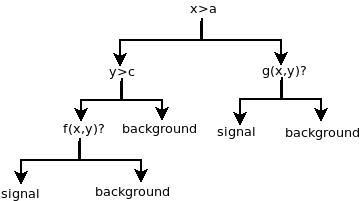
\includegraphics[width=10cm, height= 6cm]{DT.png}
    \caption{A simple decision tree for a hypothetical signal selection such that an extra parameter $g(x,y)$ is present within the algorithm. In Section \ref{sec:cut}, the partition criteria such as $x$ and $f(x,y)$ in cut-flow analysis were physically motivated and transparent. The algorithm makes this process somewhat of a black-box, making direct physical interpretations challenging.}
    \label{fig:tree}
\end{figure}

There are many tree-based methods that vary in the data sampling method and how a loss-function is minimized. In the case of EGB models, it is an extension to the \textit{Gradient Boosted Machine (GBM)} developed by Jerome Friedman \cite{friedman2001greedy}. \textit{Boosting} is an iterative algorithm in which an ensemble of weak models\footnote{A weak model consists of a small decision tree that is not an effective approximation to the data of interest.} are built sequentially, correcting its previous model through re-weighting. This leads to a final model that is highly representative of our data. Gradient boosting, extends this idea such that a differentialble loss-function's gradient (known as gradient descent) allows the errors to reduce locally, until the error is as close to zero as possible. EGB/XGBoost adds to the features of regular GBMs with weighted quantile splittings and its ability to manage sparse\footnote{Since there are no missing entries in this project, the data is not sparse, or rather, it is `dense'.} data, incorporating parallel computing to achieve faster computation time compared to regular GBM algorithms \cite{chen2016xgboost}. By also including regularization, a method to avoid overfitting by adding penalty terms to the loss-fucntion, we were able to make its predictive power more reliable. \\
%-------------------------------------------------------------------------%
\section{Metrics for model performance}
\label{sec:metrics}
The performance of a classifier can be summarized into a single table known as a confusion matrix. Displayed in Table \ref{tab:ConfMat}, a confusion matrix visually shows the distribution of correctly and incorrectly classified points within the dataset. The correctly classified signal and background events are the True Positives (TP) and True Negatives (TN), respectively. Likewise, the incorrectly classified signal and background events are the False Negatives (FN) and False Positive (FP), respectively. The accuracy of the classifier is given by (TP+TN)/N and in a regression setting such as those in xgboost, a cut-off varies this value by a slight margin. Choosing the ideal cut-off is more important than achieving high accuracy, as we wish to maximize the signal-to-background ratio (SBR)\footnote{The signal-to-background ratio is defined to be the proportion of signal over the proportion of background events. In our analysis, we look to the luminosity-normalized TP and FP rates for signal and background respectively.}\\

% Confusion matrix template
\begin{table}[htbp]
    \centering 
    \begin{tabu}{c|[2pt]c|c|c|c}
        \multicolumn{2}{c}{}&\multicolumn{2}{c}{Predicted}&\\
        \tabucline[2pt]{3-5}
        \multicolumn{2}{c|[2pt]}{}
        &\multicolumn{1}{c|}{Background} &\multicolumn{1}{c|[2pt]}{Signal} &\multicolumn{1}{c|[2pt]}{Total}\\
        \tabucline[2pt]{2-5}
        \multirow{\items}{*}{\rotatebox{90}{Simulated}}
        &\multicolumn{1}{c|[2pt]}{Background} & \multicolumn{1}{c|}{TN} & \multicolumn{1}{c|[2pt]}{FP} & \multicolumn{1}{c|[2pt]}{TN$+$FP} \\
        \cline{2-5}
        \multicolumn{1}{c|[2pt]}{}& \multicolumn{1}{c|[2pt]}{Signal} & \multicolumn{1}{c|}{FN} & \multicolumn{1}{c|[2pt]}{TP} & \multicolumn{1}{c|[2pt]}{FN$+$TP} \\
        \tabucline[2pt]{2-5}
        \multicolumn{1}{c|[2pt]}{} & \multicolumn{1}{c|[2pt]}{Total} & \multicolumn{1}{c|}{TN$+$FN} & \multicolumn{1}{c|[2pt]}{FP$+$TP} & \multicolumn{1}{c|[2pt]}{N}\\
        \tabucline[2pt]{2-5}
    \end{tabu}
    \caption{A confusion matrix for truth (simulated) and predicted labels and its components. The diagonal components are the correctly classified background (TN) and signal (TP) events. The off-diagonal components are the mis-classified background (FP) and signal (FN) events. }
    \label{tab:ConfMat}
\end{table}

An evaluation metric presented by the Higgs Challenge \cite{adam-bourdarios_learning_2014} is the \textit{approximate median significance (AMS)}, given by Equation \ref{eq:AMS}
\begin{equation}
    \text{AMS} = \sqrt{2\Big((s+b+b_r)\ln\Big(1+\frac{s}{b+b_r}\Big)-s\Big)}
    \label{eq:AMS}
\end{equation}
where $s$ and $b$ are the \textit{luminosity-normalized} TP and FP rates, respectively, and $b_r$ is a constant regularization term set at 10, found through preliminary results in the Higgs Challenge. Adding the regularization term places a bias toward larger selection regions, thus reducing the variance in the AMS value obtained. In order to obtain $s$ and $b$, we follow Equation (\ref{eq:N})
\begin{equation}
    s(b) = N_{s(b)}\times \epsilon_{s(b)} 
    \label{eq:N}
\end{equation}
where $N_{s(b)} = \sigma \int L(t) dt = \sigma \times 137$ \cite{thomson2013modern} is the number of expected events, and $\epsilon_{s(b)}=\text{TP(FP)}/\text{N}$ is the efficiency of the classifier given a dataset of size N, where in our case, would be a third of each dataset partitioned as our test set. \\

The Gaussian significance discovery, discussed briefly in Section \ref{sec:freqStat}, with an estimated standard deviation\footnote{The standard deviation is actually given by $(n-\mu_b)/\sqrt{\mu_b}$ as the Poisson fluctuation of the background has a standard deviation of $\sqrt{\mu_b}$. Here, $n$ is the number of events and $\mu_b$ is the mean of the background. These numbers are replaced with their empirical counterparts: $s+b$ and $b$ respectively.} of $s/\sqrt{b}$ only hold when $s \ll b$ and $b\gg1$. This is not true in practice, therefore we turn to an approximate measure such as the AMS. 
%This measure is a derivation of the significance Z given by Equation (\ref{eq:Z})
%\begin{equation}
%    \text{Z} = \sqrt{2\Big( n\ln\Big(\frac{n}{\mu_b}\Big)-n+\mu_b\Big)}
%    \label{eq:Z}
%\end{equation}
%where $n$ is the number of events and $\mu_b$ is the mean of the background, requiring that $n>\mu_b$. The values $n$ and $\mu_b$ are replaced by $s+b$ and $b$ in Equation (\ref{eq:AMS}), respectively. Traditionally, the Z significane at $Z=5$ corresponds to a $p$-value of less than $2.9\times10^{-7}$, sufficient to claim a discovery \cite{adam-bourdarios_learning_2014}. However, the regularization term $b_r$ is equal to zero in this setting, thus differing this significance of values given by either equations. \\
%-------------------------------------------------------------------------%
%\section{}


%-------------------------------------------------------------------------%